%%%%%%%%%%%%%%%%%%%%%%%%%%%%%%%%%%%%%%%%%%%%%%%%%%%%%%%%%%%%%%%%%%%%%%%%%%%%%%%%
%% MASTER'S THESIS                                                            %%
%%                                                                            %% 
%% Title (en): Mining Parallel Corpora from the Web                           %%
%% Title (sk): Rafinácia paralelných korpusov z webu                          %%
%%                                                                            %%
%% Author: Bc. Jakub Kúdela                                                   %%
%% Supervisor: Doc. RNDr. Irena Holubová, Ph.D.                               %%
%% Consultant: RNDr. Ondřej Bojar, Ph.D.                                      %%
%%                                                                            %%
%% Academic year: 2015/2016                                                   %%
%%%%%%%%%%%%%%%%%%%%%%%%%%%%%%%%%%%%%%%%%%%%%%%%%%%%%%%%%%%%%%%%%%%%%%%%%%%%%%%%

\chapwithtoc{Introduction}
\label{chapter:introduction}

Statistical machine translation (SMT)~\cite{Koehn09} is the most popular machine translation (MT) paradigm today. This approach to MT is preferred in organizations like Google or Microsoft, which play significant roles in an applied field where heavily used translation systems are deployed for the whole world to use. SMT utilizes statistical models for the translation. These models are trained on vast amounts of both \textit{monolingual data} and \textit{parallel data}, i.e.\ texts translated by humans.

The monolingual data help the system to understand what the target language should look like while the parallel data help the system to learn to translate smaller segments of one language into another. Monolingual data, also known as \textit{text corpora}, can be described as a simple text in a single language. Parallel data, also known as \textit{parallel text corpora}, \textit{bilingual text corpora} (in the bilingual case) or simply \textit{bitext}, are collections of sentence pairs, the sentences being of different languages, where one sentence is a translation of the other. One example of parallel texts in the human history is the famous Rosetta Stone (see Figure~\ref{figure:rosetta_stone}). The discovery of this artifact, which contained the same decree inscribed in Hieroglyphic, Demotic and Greek, led to deciphering and understanding of the extinct Hieroglyphic writing.

\begin{figure}[!htb]
	\centering
	\caption{Rosetta Stone}
	\label{figure:rosetta_stone}
	\vspace{1em}
	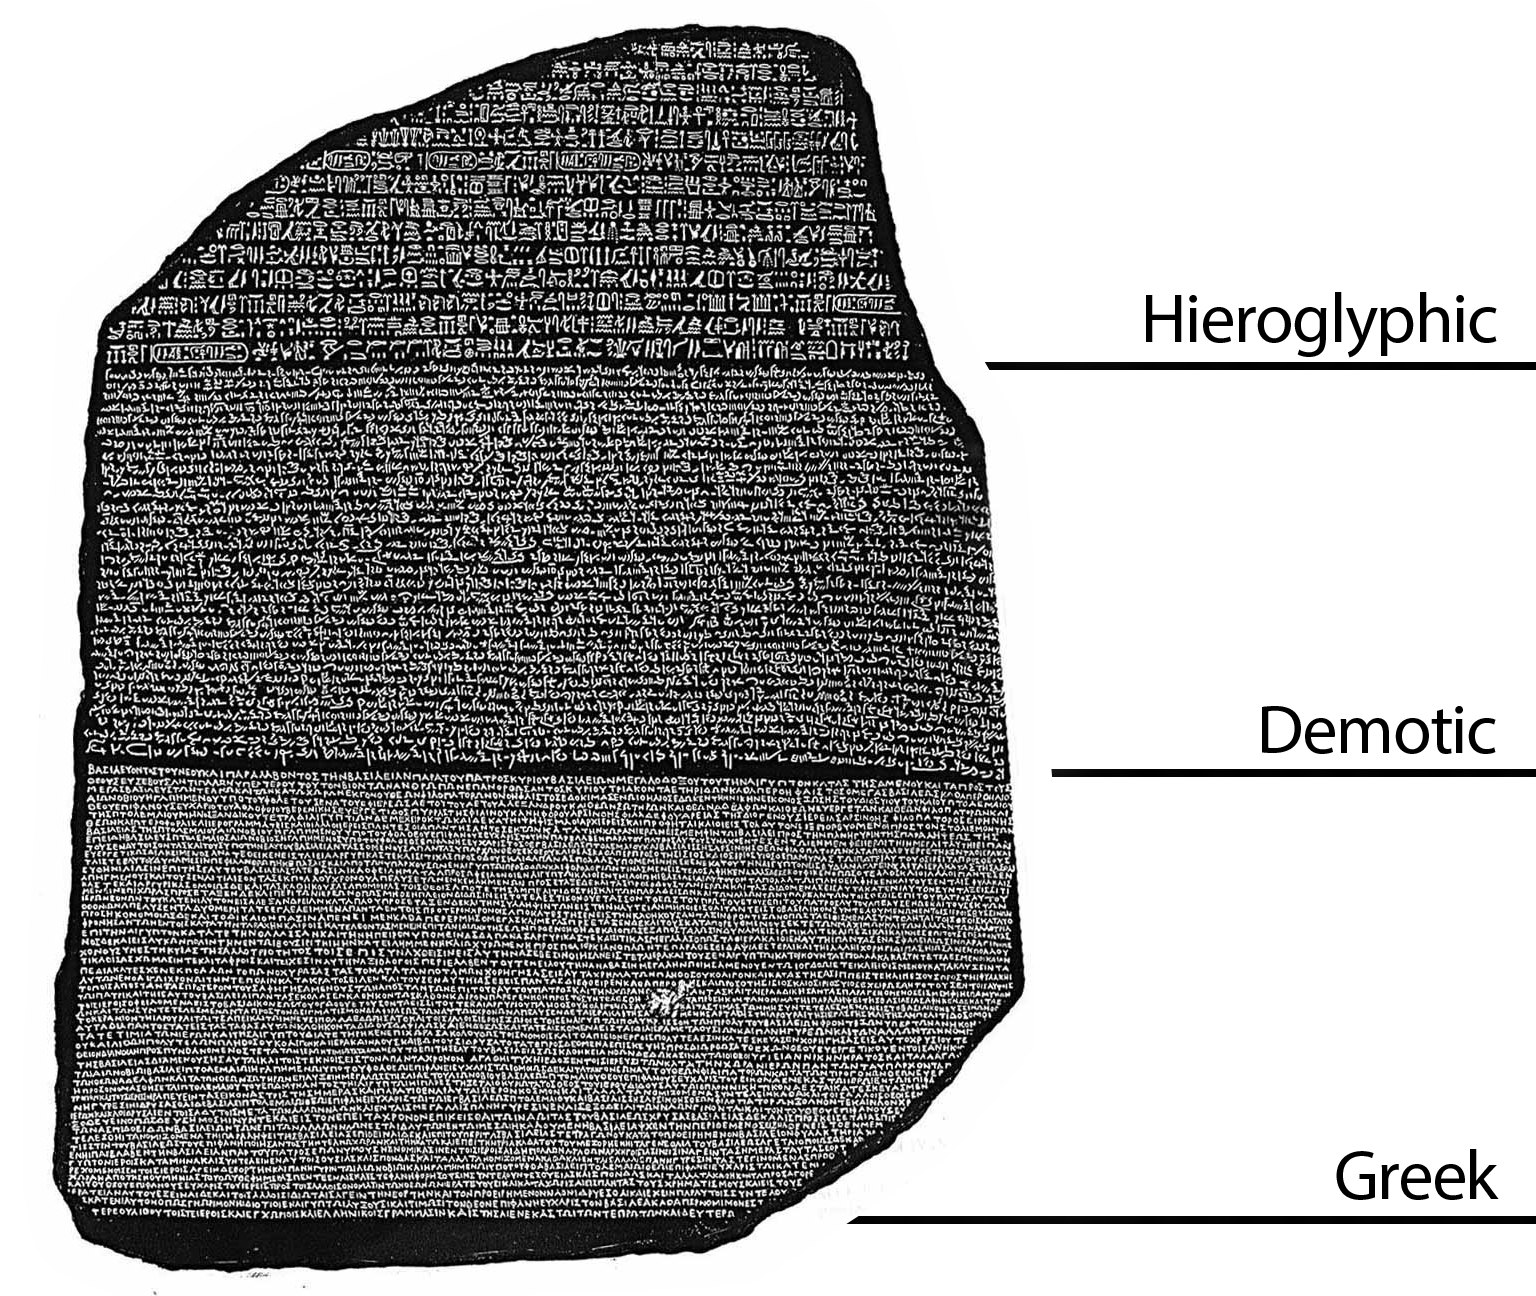
\includegraphics[width=0.6\textwidth]{images/rosetta_stone.png}
\end{figure}

The existence of parallel data is the most important prerequisite for building an effective SMT system. Today there exist a plenty of both monolingual and sentence-aligned parallel data. Such a collection of corpora is for example OPUS~\cite{Tiedemann12}. One of the richest sources of the parallel data included in OPUS are texts produced by government organizations, such as the European Parliament Proceedings, which are being translated into each of the 23 official languages of the European Union. Other important sources we could mention are movie subtitles, books, news websites, or localization files of computer software. 

We believe that the web is a potential source of considerable amounts of parallel data generated not only by well-known organizations like the European Parliament but also by organizations of smaller sizes and by individuals. In the field of SMT there is also motivation and need for acquisition of parallel data from various domains. To illustrate this motivation, an SMT system trained on just the parallel data from the European Parliament Proceedings may seem cumbersome in translation of standard speech language because of the formal nature of the training data. We assume that by mining parallel data from the web, we can obtain useful parallel corpora which would also reflect the natural distribution of domains.

\section*{Goals}

The main goal of our thesis is to propose a method for solving the task called \textit{bilingual document alignment} applicable in the field of mining parallel data from the web. This problem can be generally stated as follows: assume we have a set of documents written in two different languages, where a document is a plain text not limited by length; it can be a sentence, a sequence of multiple sentences, or even a single word. The solution of this task is a collection of all such pairs of documents in different languages that are mutual translations of each other.

We would like to distinguish our method by taking a different approach than the one shared by many others. The majority of methods developed in the field primarily use the structure of the web pages in the alignment process. We believe that by performing structure similarity filtering, we can lose a considerable part of parallel data. 

The aim is to propose a more generic method, not based on page structure comparison. The method is expected to find bitexts located on pages not at all similar in structure. In other words, our motivation is to find the parallel segments, i.e.\ paragraphs we consider as input documents to our method, contained on a given bilingual web domain, regardless of the structure of its web pages. By moving to these finer units, we also have to rely more on the actual content of the paragraphs. To overcome the well-known problems of data sparseness, we plan to use currently popular models like \textit{word2vec}~\cite{Mikolov13a}\cite{Mikolov13b}\cite{Mikolov13c}, and to deal with the possibly large amount of input documents, we intent to make use of recently studied strategies for \textit{locality-sensitive hashing}~\cite{Charikar02}\cite{Andoni08}.

Any finer alignment of the documents, such as sentence alignment, is beyond the scope of our work. The methods for achieving sentence alignment for a document-aligned parallel corpus are well examined~\cite{Tiedemann11} and can be easily applied to the output of our method. 

Moreover, our particular requirements for the target method are scalability and reasonable behavior on noisy and sparse data, where only some of the input documents will have a pair. Both these requirements are needed when processing data from the web. It is also important to mention that the method is expected to be supervised, which means it depends on the provided a priori knowledge in the form of an already existing sentence-aligned bilingual text corpus that is used in the training process. However, this does not mean that the training corpus needs to cover every single word contained in the actual input documents. 

Another goal of this work is to perform experiments with the proposed method and present their results. Our experiments are solely focused on the Czech--English~\cite{Bojar12_1} language pair. The first experiment is carried out using CzEng 1.0~\cite{Bojar12_2}---a Czech--English sentence-aligned parallel corpus. This way we can measure the quality of the results automatically. The second experiment uses more realistic, noisy data provided by the Common Crawl Foundation~\cite{CommonCrawl}---a non-profit organization with the goal of democratizing access to web information. It produces and maintains an open repository of web-crawled data that is universally accessible and analyzable.

\section*{Outline}

The rest of this thesis is organized as follows. Chapter~\ref{chapter:related_work} introduces the related work in this field, covering similar approaches that have been already explored. They can still serve as an inspiration for the potential extension of ideas covered in the thesis. In Chapter~\ref{chapter:background_work_and_prerequisities} we discuss technologies used in our work, together with reasoning and motivation for their selection. Chapter~\ref{chapter:proposed_method} contains a detailed description of the proposed method with all implementation details. Chapter~\ref{chapter:prealigned_data_czeng_experiment} describes the experiment done on the CzEng 1.0 corpus. In Chapter~\ref{chapter:web_data_common_crawl_experiment} the experiment done on the Common Crawl dataset is explained, along with a way how to mine parallel corpora from the vast amounts of real-world web data. The final chapter concludes the discussion and suggests potential directions of future work.